%Sonos - They solved the problem for their wireless speakers
%The speakers streams the music individually, not the phone to speakers
%RTP(RTSP) -- Protocols for data streams
	%RTP is for audio and video streams
	%RTSP is usecd to control streaming media services, they are used together, RTP also uses H.323  (utube)
	%http://stackoverflow.com/questions/19620219/does-youtube-stream-videos-via-tcp
	%Build on UPD
%RTCP
%RTMP
%MMS
%Smooth Streaming
%HLS (twitch)
%https://www.reddit.com/r/Twitch/comments/2cnztw/why_does_twitch_have_a_delay/
%http://www.streamingmedia.com/Articles/Editorial/What-Is-.../What-Is-a-Streaming-Media-Protocol-84496.aspx
%DASH(Netflix used)
%https://www-users.cs.umn.edu/~viadhi/netflix.pdf
%Spotify uses its own propriatary
%https://blogs.commons.georgetown.edu/cctp-797-fall2013/archives/557
%http://pansentient.com/2011/04/spotify-technology-some-stats-and-how-spotify-works/
%https://www.csc.kth.se/~gkreitz/spotify/kreitz-spotify_kth11.pdf

%http://applian.com/replay-media-catcher/support/supported_protocols5

%Conclusion: synchronized streaming services seem to be generally using propriatary software

%https://snarfed.org/synchronizing_mp3_playback  --- this guy did it

%SqueezeBox - http://wiki.slimdevices.com/index.php/SlimProto_TCP_protocol - propriatary protocol



\section{Technologies}
In this section we take a closer look at streaming and split this into two primary types of streaming, video and audio.
As we are focused on audio streaming, services and solutions in this field are the most important ones, however video streaming services are also mentioned in order to compare the two.
Furthermore we separate Audio streaming and multi-room audio systems, i.e. synchronized audio streaming using multiple devices, as this is a special case of audio streaming and also happens to be closely related to our problem.

\subsection{Audio Streaming}
Streaming music is a common way of listening to music with services such as Spotify making a large selection of music available through a subscription service.
A key part in streaming audio is the streaming protocol, to this end Spotify previously used peer-to-peer networking in order to handle the demand.\cite{spotify1}
However, demand is not a concern for us, the streaming protocol used is.
As for streaming protocol, Spotify uses their own proprietary protocol, as is represented on \cref{fig:spotifyOverview}.\cite{spotifySlides} %I kilden skriver de også at de går efter en unified backend protocol istedet for at dvs. de er nok 100% propriatary nu, should this be mentioned? im not sure it matters too much

Aside from the fact that Spotify uses a proprietary protocol not much else about the protocol is public.
Spotify is not the only streaming service out there, another popular service is Airplay.
Airplay also use their own proprietary protocol, Remote Audio Output Protocol, which is based on \acl{RTSP}.
In fact the general impression received is that the audio streaming services use proprietary protocols.

\begin{figure}[h!]
    \centering
    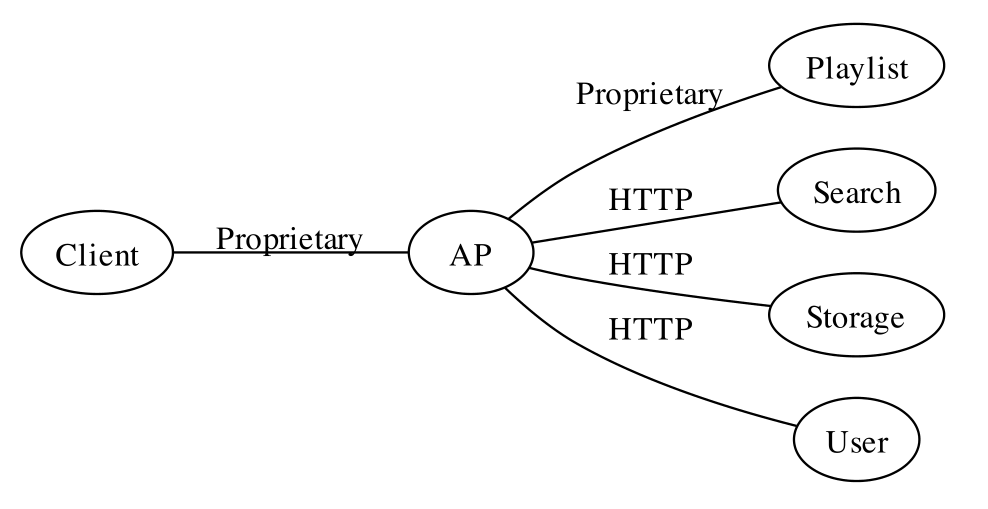
\includegraphics[width=0.7\textwidth]{img/spotifyOverview.png}
    \caption{High level overview of Spotify from 2011 \cite{spotifySlides}}
    \label{fig:spotifyOverview}
\end{figure}

%Spotify - propriatary
%Pandora - unknown
%Airplay -  Remote Audio Output Protocol (RAOP), a proprietary variant of RTSP/RTP

\subsection{Video Streaming}
For streaming video there are a variety of streaming services out there, these are generally of two types, livestreaming services such as twitch, which do not just stream from a server, but streams live from another client.
The other type streams from a server, such as Netflix which allow for streaming of movies and tv-shows.
In contrast to the audio streaming services the video streaming services do not seem to be relying on proprietary streaming protocols.

Netflix uses \acl{DASH}, Twitch uses \acl{HLS} and previously used \acl{RTMP} which they still support, and Youtube uses \acl{RTSP}.\cite{netflix}\cite{twitch}\cite{youtube}
Neither of these three streaming services use the same protocol, and all three are in the top of the market.
A difference between perhaps Netflix and twitch may have been because they are slightly different, but Youtube and twitch also offer the same services and yet use different protocols.
This gives the impression that there must be a considerable difference between audio and video streaming when it comes to the streaming protocol.
%Netflix -- DASH
%Twitch -- HLS&RTMP
%Youtube -- RTSP

\subsection{Multi-Room Audio Systems}
Beyond streaming protocols there is another technology which closely relates to our problem, namely Multi-Room Audio.
Multi-Room Audio is fairly self-descriptive, it provides audio to several rooms, this audio however is synchronized.
While there are several ways of making a Multi-Room Audio solution for a home, predominately the technology is developed and provided by speaker manufacturers.
Several manufacturers provide this service to a degree but one manufacturer in particular is leading the technology and build their entire brand around it, Sonos.

It is Sonos' proprietary network software alongside their hardware that have kept them at the top of the market.
Sonos' own mesh network was developed due to WiFi not being of sufficient at the time when Sonos started development, this however is no longer the case is can be seen my both their competitors such as Bose, and their own technology which now also supports standard WiFi, although their own network is still more reliable. %https://www.theregister.co.uk/2014/09/02/sonos_ditches_music_streaming_bridges/
It is their proprietary peer-to-peer mesh network, aptly named SonosNet, which makes them top of the market. %https://en.wikipedia.org/wiki/Sonos
The market is still very competitive and as such information on the specific technologies and software is scarce, beyond knowing it is proprietary.

%Sonos
%enon
%Pure
%Samsung
%All the speaker producing companies -- Sonos Propriatary, others not looked in to yet.


\subsection{Conclusion}\fxnote{Tænker dette skal nok samles i et større SOTA conclusionsafsnit hvor der opsamles på alle dele frem for at have en conclusion i hver subdel af sota}
From the information gathered in this section we derive conclusions to help us formulate the problem and elicitate requirements in order to solve that problem.
From the audio streaming segment we can see that there is a tendency to use proprietary software, this gives us the impression that there are certain requirements which the well known streaming protocols do not fully support. 

We know specifically from AirPlay that their solution is based on \ac{RTSP}, thus there are some elements to the protocol that works just fine but simply does not fulfill all of AirPlays requirements.
We want to extend beyond simple streaming of audio to use multi-room audio technology, i.e. synchronize across devices. 
Our insight into this field show that whilst Sonos use their own network, SonosNet, WiFi and Bluetooth both work just fine, as Sonos' competitors use these, and Sonos themselves also support standard WiFi.
As for their streaming protocol, similarly to the audio streaming services we know no more than that it is proprietary.
Our insight into video streaming may help shed some light on as to why proprietary software is used rather than the more common streaming protocols, in this field the companies use the common ones, and not one in particular.

This lets us conclude that the difference in requirements for audio compared to video streaming is what is causing audio focused companies to use proprietary streaming protocols.
Some of these differences may include latency, file size, bit rate, etc.
As such going forward we must explore how these factors affect the streaming protocols in concern to audio to ascertain which protocol to use, and whether we should fiddle with the protocols.




%Audio generally uses some sort of propriatary software, latency perhaps?
%Multi-Room Audio done succesfully is generally done by speaker manufactorers using propriatary software alongside their own hardware(Sonos only works with Sonos)
%Video streaming, uses the well known protocols such as Hls,Dash and RTSP

%=The difference between audio and video streaming is causing audio streaming to use propriatary software protocols?
%So what is the major differences? --> File sizes, bit rate.
%            A movie can buffer for a few minutes before starting to not lag during the movie, users understand this
%            A song cannot buffer for a few minutes before starting, users will notice and dislike this
%                    Assumption: Propriatary software is used to reduce latency such that a song can start asap? or to fix some other criteria that the basic protocols dont live up to.

%This is propriatary because there are no standard protocols for controlling several speakers at once in a synchronized manner(This is very hard to source, reviews focus on the tech, and sound quality, not software - protocols are rarely mentioned in more than 1 line and software is never the focus of speaker reviews)




%RandomLinks:
    %http://www.trustedreviews.com/opinions/the-ultimate-multi-room-audio-guide
    %http://www.techhive.com/article/3034868/speakers/yamaha-musiccast-review-this-multi-room-audio-system-is-better-than-expected.html
    %https://www.cnet.com/news/bose-soundtouch-throws-down-multiroom-audio-gauntlet-to-sonos/
    %http://www.danplanet.com/blog/2014/11/26/multi-room-audio-with-multicast-rtp/
    %http://www.pocket-lint.com/news/136462-multi-room-audio-what-is-it-and-what-are-your-options

    %https://attackllama.com/2014/04/sonos-like-synchronised-streaming-part-2/